% Short paper for the language-driven grasp detection interview task.
% Template link in the task PDF: https://www.overleaf.com/latex/templates/cvpr-2022-author-kit/qbmjsdxryffn
% The bundled style and bibliography files match cvpr-org/author-kit at
% a2369342011145be8c85e5ad21a9b61f9fa53473.
\documentclass[10pt,twocolumn,letterpaper]{article}
\usepackage{cvpr}
\usepackage{times,amsmath,amssymb,graphicx,booktabs}
\usepackage{tikz}
\usetikzlibrary{positioning,arrows.meta}
\definecolor{cvprblue}{rgb}{0.21,0.49,0.74}
\usepackage[pagebackref,breaklinks,colorlinks,allcolors=cvprblue]{hyperref}
\def\confName{Technical Report}
\def\confYear{2026}
\title{Same-Image Prompt Ranking for Language-Driven Grasp Detection: A Controlled Study}
\author{Yuquan Wang\\\url{https://github.com/labron23wyq/swapgrasp}}

\begin{document}
\maketitle
\begin{abstract}
Language-driven grasp detection must select a grasp on the object or part named by text. We add symmetric same-image support ranking to a ResNet-18/FPN detector conditioned by frozen CLIP. On an image-disjoint subset, three matched seeds give Top-1 success of 53.18\% for the baseline and 52.64\% for the proposed objective; paired image-bootstrap intervals do not establish a gain. A separate follow-up gives 50.66\% for candidate reranking versus 50.38\% for its detector baseline, again with intervals spanning zero. We report a diagnostic study, not a claim of reliable improvement.
\end{abstract}

\section{Introduction}
Given an RGB image and a language instruction, the task predicts a planar grasp rectangle $(x,y,w,h,\theta)$. A plausible grasp can still target the wrong object or part. Prior work studies language-conditioned detection on Grasp-Anything++~\cite{Vuong2024language}, referring grasp synthesis in clutter~\cite{Tziafas2023language}, and mask-guided attention~\cite{VanVo2024language}.

We test whether explicit same-image prompt switching helps distinguish co-occurring targets. This work contributes a compact objective and controlled evaluation, not a new backbone:
\begin{itemize}\setlength{\itemsep}{0pt}\setlength{\topsep}{2pt}
\item Same-image target-versus-distractor ranking for paired prompts.
\item Matched multi-seed evaluation with geometric and pair-level metrics.
\item Follow-up sampling and ranking diagnostics with uncertainty reported.
\end{itemize}

\section{Method}
\begin{figure}[t]
\centering
\resizebox{\linewidth}{!}{%
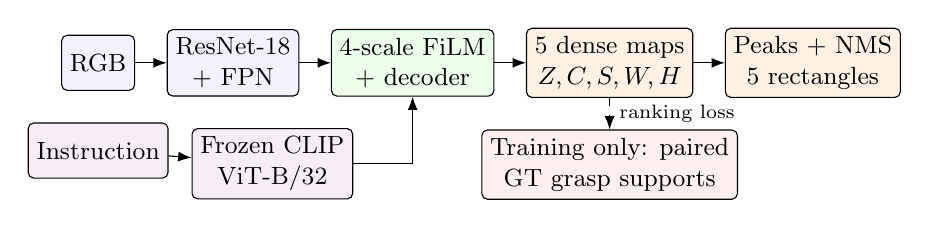
\begin{tikzpicture}[>=Latex,box/.style={draw,rounded corners=2pt,align=center,font=\small,minimum height=7mm,inner sep=3pt},node distance=4mm and 4mm]
\node[box,fill=blue!5] (rgb) {RGB};
\node[box,fill=blue!5,right=of rgb] (vision) {ResNet-18\\+ FPN};
\node[box,fill=green!8,right=of vision] (fusion) {4-scale FiLM\\+ decoder};
\node[box,fill=orange!10,right=of fusion] (maps) {5 dense maps\\$Z,C,S,W,H$};
\node[box,fill=orange!10,right=of maps] (decode) {Peaks + NMS\\5 rectangles};
\node[box,fill=violet!7,below=of rgb] (text) {Instruction};
\node[box,fill=violet!7,below=of vision,xshift=5mm] (clip) {Frozen CLIP\\ViT-B/32};
\node[box,fill=red!6,below=of maps] (support) {Training only: paired\\GT grasp supports};
\draw[->] (rgb)--(vision);\draw[->] (vision)--(fusion);\draw[->] (fusion)--(maps);\draw[->] (maps)--(decode);
\draw[->] (text)--(clip);\draw[->] (clip)-|(fusion);
\draw[dashed,->] (maps)--node[right,font=\scriptsize]{ranking loss}(support);
\end{tikzpicture}}
\caption{Detector and training-only prompt-switch supervision. At inference, only the image and instruction are used.}
\label{fig:architecture}
\end{figure}

\paragraph{Detector.} An ImageNet-initialized ResNet-18 and feature pyramid produce four visual scales. A frozen CLIP ViT-B/32 text encoder conditions each scale through FiLM, $(1+\gamma(t))\odot F+\beta(t)$. A decoder predicts five $320\times320$ maps: quality logits $Z$, doubled-angle components $(C,S)$, and log width and height $(W,H)$. The doubled angle represents the gripper's $\pi$-periodic symmetry. We decode local peaks, apply rotated non-maximum suppression, and retain five candidates. Inference uses no target mask or ground truth.

\paragraph{Prompt-switch loss.} For two instructions $t_a,t_b$ naming distinct objects in the same image, let $P_a,P_b$ be their disjoint grasp-center support pixels. Pair construction checks object masks and grasp annotations offline; the loss acts on predicted quality logits. We summarize a support by normalized log-sum-exp:
\begin{equation}
r(Z,P;\tau)=\tau\log\!\left(\frac{1}{|P|}\sum_{u\in P}\exp(Z(u)/\tau)\right).
\end{equation}
The symmetric objective is
\begin{equation}
\begin{split}
\mathcal{L}_{\rm swap}=\tfrac12[&\operatorname{softplus}(m-r(Z_a,P_a)+r(Z_a,P_b))\\
 &+\operatorname{softplus}(m-r(Z_b,P_b)+r(Z_b,P_a))].
\end{split}
\end{equation}
It rewards each prompt's own support over the competing support, in both directions. We use $m=0.2$, $\tau=0.25$, and $\mathcal{L}=\mathcal{L}_{\rm quality}+\mathcal{L}_{\rm geometry}+\lambda\mathcal{L}_{\rm swap}$, with $\lambda=0$ for the baseline and $0.1$ for SwapGrasp.

\begin{table*}[t]
\centering\scriptsize
\setlength{\tabcolsep}{3.2pt}
\begin{tabular}{llrrrrr}
\toprule
Study & Method & Top-1 & Top-5 & Strict@1 & VeryStrict@1 & Pair@1\\
\midrule
Primary, 3 seeds & Baseline & 53.18$\pm$1.43 & 82.19$\pm$0.31 & 45.31$\pm$1.42 & 20.22$\pm$0.51 & 35.80$\pm$4.89\\
& SwapGrasp & 52.64$\pm$1.36 & 82.70$\pm$2.02 & 43.62$\pm$2.01 & 17.87$\pm$3.52 & 31.04$\pm$5.71\\
\midrule
Follow-up, 2 seeds & Original & 50.38$\pm$0.90 & 83.12$\pm$0.14 & 40.76$\pm$1.31 & 11.43$\pm$2.92 & 25.60$\pm$2.75\\
& Balanced & 50.00$\pm$1.72 & 80.40$\pm$0.05 & 42.25$\pm$0.43 & 17.93$\pm$1.27 & 18.11$\pm$1.91\\
& Hard Swap & 49.70$\pm$1.65 & 80.32$\pm$0.20 & 41.26$\pm$2.37 & 18.94$\pm$0.07 & 18.71$\pm$6.56\\
& Reranker & 50.66$\pm$1.02 & 80.40$\pm$0.05 & 42.38$\pm$0.20 & 18.35$\pm$1.72 & 18.86$\pm$2.12\\
\bottomrule
\end{tabular}
\caption{Test success in percent (mean $\pm$ seed standard deviation). The two studies use different splits and are not pooled; follow-up images overlap the earlier training pool. Reranking preserves the five proposals, so its Top-5 equals Balanced.}
\label{tab:results}
\end{table*}

\section{Experiments}
\paragraph{Primary matched study.} The image-disjoint split has 7,477/704/605 train/validation/test images and 25,701/2,486/1,960 instructions. We quarantine 362 unit-ambiguous annotations. Test includes 189 valid pairs from 36 images. Both models use identical initialization and per-seed schedules, seeds 42/123/3407, batch 256, and 5,050 steps (64 paired instruction pairs per batch). Validation Top-1 selects checkpoints.

\paragraph{Metrics.} Standard success is rotated IoU $>0.25$ and angle error $<30^\circ$; Strict and VeryStrict use $(0.50,15^\circ)$ and $(0.75,10^\circ)$. Top-5 checks any of five candidates; Pair@1 requires both prompts to succeed at Top-1. Values are mean $\pm$ sample standard deviation across seeds. We use 1,000 image-cluster bootstrap resamples.

\paragraph{Results and follow-up.} In the primary study, SwapGrasp changes Top-1/Strict@1/VeryStrict@1/Pair@1 by $-0.54/-1.69/-2.35/-4.76$ points; Top-5 changes by $+0.51$. Seed-wise Top-1 changes are $-1.63$, $+1.99$, and $-1.99$; every image-bootstrap interval includes zero.

The follow-up uses 6,580/353/351/897 train/validation/rankfit/test images and 3,128 test instructions. Test images came from the previous training pool, and the variants were motivated by earlier results, so this is not independent confirmation. Reranking gains 0.66 points over Balanced but only 0.27 over Original; both Original comparison intervals include zero. The reranker uses labels from 351 extra rankfit images, so its effect is not isolated. Hard Swap is seed-sensitive; stricter geometry can improve while Top-5 and paired success fall.

\paragraph{Limitations and conclusion.} This filtered Grasp-Anything++ subset has noisy language labels; continuous polygon IoU is not aligned sample-by-sample with the official raster evaluator, and no robot trial was run. Current evidence does not show a reliable Top-1 gain. New-scene evaluation, verified referring labels, and robot trials are needed.

{\small
\begin{samepage}
\bibliographystyle{ieeenat_fullname}
\bibliography{references}
\end{samepage}
}
\end{document}
